%!TEX root = main.tex

\subsubsection{Semantics of $\AOAMASS$}\label{sec:aoamass}

It turns out that the semantics of $\AOAMASS$ is still complicated due to the complex interplay between launch modes and intent flags. Therefore, in the sequel, we separate the concerns further and consider the two sub-models of $\AOAMASS$, namely $\LMAOAMASS$ and $\IFAOAMASS$, which focus on launch modes and intent flags of $\AOAMASS$ respectively. 
More precisely, 
%
\begin{itemize}
\item an $\LMAOAMASS$ is an $\AOAMASS$ where all the transition rules $A \xrightarrow{\alpha(\phi)} B$ (except $\back$) satisfy that $\phi = \bot$, 
\item an $\IFAOAMASS$ is an $\AOAMASS$ where all the transition rules $A \xrightarrow{\alpha(\phi)} B$ (except $\back$) satisfy that $\lmd(A) = \STD$. 
\end{itemize}
%
To ease the understanding, in the main text, we shall only define the formal semantics of the two sub-models $\LMAOAMASS$ and $\IFAOAMASS$, and omit the definition of the formal semantics of $\AOAMASS$,
%delegate the definition of the formal semantics of $\AOAMASS$ to the appendix, 
since the definition of the semantics of $\AOAMASS$ is rather tedious and we think that $\LMAOAMASS$ and $\IFAOAMASS$ are already sufficient to understand the meanings of the launch modes and intent flags. 

To simplify the presentation, in $A \xrightarrow{\alpha(\phi)} B$, we assume that $\alpha$ is $\startactivity$. The definition of the semantics for the case that $\alpha$ is $\finishstart$ can be found in the appendix. 

%%%%%%%%%%%%%% Semantics of LMAOAMASS %%%%%%%%%%%
%%%%%%%%%%%%%% Semantics of LMAOAMASS %%%%%%%%%%%
%%%%%%%%%%%%%% Semantics of LMAOAMASS %%%%%%%%%%%

\smallskip
\noindent {\bf Semantics of $\LMAOAMASS$}.
\smallskip

We start with the semantics of $\LMAOAMASS$ and assume that $\Mm$ is an $\LMAOAMASS$. 
We first introduce some notations. 

%Before defining the semantics of $\LMAOAMASS$ and $\IFAOAMASS$, we introduce some notations. 

%In this case, we consider activities as atomic objects, so we only consider transaction rules of the form $\back$ and $A\xrightarrow{\alpha(\phi)}B$.}
%\subsection*{Intuitions.}
%The intuitions of the transition rules %(except $\back$) 
%are as follows.  
%\begin{itemize}
%	\item $\startactivity(A, \phi)$ denotes the action where the activity $A$ is started with the intent flag $\phi$.
%	
%	\item $\finishstart(A, \phi)$ is the same as $\startactivity(A, \phi)$, except that the current activity is popped after starting $A$.
%\end{itemize}

\paragraph{Tasks and configurations}
A \emph{task} of $\Mm$ is represented by its activity stack and is encoded as a word $S= [A_1, \cdots, A_n] \in \act^+$, with $A_1$ (resp. $A_n$) as the top (resp. bottom) activity of $S$, $n$ is called the \emph{height} of $S$. 
% We define the \emph{affinity of a task} $S$, denoted by $\aft(S)$, to be $\aft(\btmact(S))$. For $S_1 \in \act^*$ and $S_2 \in \act^*$, we use $S_1 \cdot S_2$ to denote the concatenation of $S_1$ and $S_2$, and $\epsilon$ is used to denote the empty word in $\act^*$. 

A \emph{configuration} of $\Mm$ is encoded as a sequence 
$\rho=(\Omega_1,\cdots,\Omega_n)$, and for each $i \in [n]$, $\Omega_i = (S_i,A_i,\zeta_i)$, $S_i\in\act^*$ is a task, $A_i\in\act$ is the real activity of $S_i$, $\zeta_i\in\{\mainflag,\STK,\SIT\}$ represents how the task $S_i$ is launched. 
% a pair $(\rho, \ell)$, where $\rho=(\Omega_1,\cdots,\Omega_n)$, and for each $i \in [n]$, $\Omega_i = (S_i,A_i,\zeta_i)$, $S_i\in\act^*$ is a task, $A_i\in\act$ is the real activity of $S_i$, $\zeta_i\in\{\mainflag,\ntkflag,\ndmflag,\SIT\}$ represents how the task $S_i$ is launched, and $\ell\in\{0,1\}$ represents the top activity is (resp. \emph{not}) launched with the intent flag $\nohflag$ if $\ell = 1$ (resp. $\ell = 0$).
% $S_i$ is (resp. not) the main task, if $b_i=1$ (resp. $b_i=0$).
% We use $\topact(\rho)$ to denote \emph{the top activity} of $\rho$, namely, the top activity of $S_1$. 
For any activity $A$, we refer to an $A$-task as a task whose real activity is $A$. 
%
The tasks $S_1$ and $S_n$ are called the top and the bottom task respectively. (Intuitively, $S_1$ is the foreground  task.) The symbol $\varepsilon$ is used to denote the empty task stack. 
The \emph{affinity of a task} is defined as the affinity of its real activity. A task $(S_i,A_i,\zeta_i)$ in $\rho$ is called an $\SIT$-task if $\zeta_i = \SIT$. 
%It turns out that the semantics of the transition rules of $\Mm$ can guarantee that for any pair of distinct tasks in $\rho$, if none of their real activities has the $\singleinstance$ (SingleInstance) launch mode, then their affinities should be different. 
%Therefore, the number of tasks in $\rho$, that is, $n$, should be no more than $|\aft(\act \setminus \act_{\singleinstance})| + |\act_{\singleinstance}|$, where $\act_{\singleinstance}$ is the set of activities with the $\singleinstance$ launch mode.

A task is called the \emph{main task} of the task stack if it is the first task that was created when launching the app. Note that the current task stack may \emph{not} contain the main task, since it may have been popped out from the task stack. This notion is introduced since the semantics of {\AMASS} is also dependent on whether the task stack contains the main task.

Let $\conf_\Mm$ denote the set of configurations of $\Mm$. The \emph{initial} configuration of $\Mm$ is $(([A_0],A_0,\mainflag))$. 
%
The \emph{height} of a configuration $\rho$ %a configuration $\rho = ((S_1, A_1), \cdots, (S_m, A_m))$ 
is defined as $\max \limits_{i \in [m]}|S_i|$, where $|S_i|$ is the height of $S_i$. By convention, the height of $\varepsilon$ is defined as $0$. 

Before presenting the formal semantics of $\LMAOAMASS$, we present its intuitions. 
%

\paragraph{Intuitions of the launch modes.}  %We explain the intuitions of the four launch modes. 
We call an activity of the launch mode $\STD$ as an $\STD$-activity, similarly for $\STP$, $\STK$ and $\SIT$. 

\begin{itemize}
\item The $\STD$ mode: When a new $\STD$-activity is started, it will be pushed into the top task. 
%
\item The $\STP$ mode: When a new activity of the $\STP$ mode is started, if the activity is already at the top of the top task, it will reuse this activity. Otherwise, a new activity will be pushed into the top task.
%
\item The $\STK$ mode: When a new activity of the $\STK$ mode is started, it will create the activity at the root of a new task or locates the activity on an existing task with the same affinity. If the activity already exists, then all the activities above it are removed from the task. Otherwise, a new activity will be pushed into the task.
%
\item The $\SIT$ mode: 
Similar to $\STK$, but if such an activity already exists, it will reuse this activity, moreover there is only one activity in the task which was created by starting the same activity.
\end{itemize}

\paragraph{Task allocation mechanism.}
The intuitions of the launch modes are actually not that precise. For instance, when a new $\STD$-activity is stated by an $\SIT$-activity, the $\STD$-activity will not necessarily be pushed to the top task. 
%For instance, an $\SIT$-task only contains one activity,  if the launch modes of the caller and callee activity are $\SIT$ and $\STD$ respectively, then the callee activity is pushed into a non-top task.
Task allocation mechanism is to specify to which task will it be allocated when an activity is launched. Via extensive experiments, we  
identify a crucial notion, i.e., real activity of tasks, 
%in Android 7.0 and later versions, 
%use an attribute of tasks called real activity, which 
which plays a pivotal role in such a mechanism. 
%The real activity of a task is 
%is the activity  which was pushed into the task---as the bottom activity---when the task is created. 
%Intuitively, $A_i$ is the activity which was pushed into the taskwhen the task $S_i$ was created.

Generally speaking, for an activity $B$  which is not to land on the top task, %then the task-searching means go in 
the following three steps will apply: (1) If there is any task whose real activity is $B$, then $B$ will be put on the task. %(search downwards from the top task). 
(2) Otherwise, if there is any task whose real activity has the same \emph{task affinity} as $B$, then $B$ will be put on the task. %first such task (search downwards from the top task). 
(3) Otherwise, a new task is created to hold $B$. In the first two cases, if there are multiple instances, the first occurrence starting from the top task will be selected. 

\paragraph{Real activity and main task.}
When the caller activity is an $\SIT$ activity and the callee activity is an $\STD$ or $\STP$ activity $B$, $B$ will \emph{not} always be pushed into the task $S_i$ which is specified according to the \emph{task allocation mechanism}. Generally speaking, the following steps will apply: (1) If the real activity of $S_i$ is \emph{not} $B$, then $B$ will be pushed into $S_i$. (2) Otherwise, if $S_i$ is the main task, that is, $\zeta_i=\mainflag$, then $B$ will be pushed into $S_i$. (If $S_i$ is not the main task, then $B$ will not be pushed.)

\smallskip

Then we introduce some auxiliary functions and predicates to be used in the formal semantics of $\LMAOAMASS$.

\paragraph{Auxiliary functions and predicates.} To specify the transition relation precisely and concisely, we define the following functions and predicates. 
Let $\rho = (\Omega_1,\cdots,\Omega_n)$ be a configuration with $\Omega_i = (S_i,A_i,\zeta_i)$ for each $i\in[n]$, and $S=[B_1,\cdots,B_m]$ be a task. 
% Let $(\rho,\ell)$ be a configuration with $\rho = (\Omega_1,\cdots,\Omega_n)$ with $\Omega_i = (S_1,A_i,\zeta_i)$ for each $i\in[n]$, and $S=[B_1,\cdots,B_m]$ be a task. 
\begin{itemize}
	%	\item $\realact(S) = A$, where $S$ is created by an action $start(A,\Ff)$
    \item $\topact(S) = B_1$, $\btmact(S) = B_m$, %~\mbox{where}~ S = A(\act^*)$
	%	\item.  %, ~\mbox{where}~ S = (\act^*)A$\push
	\item $\toptsk(\rho) = S_1$,  %this is the foreground task
        $\topact(\rho) = \topact(\toptsk(\rho))$, %, where $S_1 = [A]\cdot S_1'$.
	
    \item $\push(\rho, B) = (([B] \cdot S_1,A_1,\zeta_1), \Omega_2, \cdots, \Omega_n)$,
    	
%	\item $\mvacttop(\rho, B)  =(([B]\cdot S'_1 \cdot S''_1,A_1,\zeta_1), \Omega_2, \cdots, \Omega_n) $, 
%        if $S_1=S'_1 \cdot[B]\cdot S''_1$ with $S'_1 \in (\act \setminus \{B\})^*$,
	%---------------------------------------------------------------------------------------------------------------
    \item $\clrtop(\rho, B) = (([B]\cdot S_1'',A_1,\zeta_1),\Omega_2,\cdots, \Omega_n)$ if $S_1=S'_1 \cdot S''_1$ with $S'_1 \in (\act \setminus \{B\})^*B$,
	
    \item $\clrtsk(\rho, B)  = (([B],A_1,\zeta_1),\Omega_2,\cdots, \Omega_n)$,
	
    \item $\mvtsktop(\rho, i) = (\Omega_i,\Omega_1,\cdots,\Omega_{i-1},\Omega_{i+1},\cdots,\Omega_n)$,

    \item $\newtsk(\rho, B, \zeta)  = (([B],B,\zeta),\Omega_1,\cdots, \Omega_n)$,
	%---------------------------------------------------------------------------------------------------------------
	
	\item $\getrealtsk(\rho, B) = S_i$ such that $i \in [n]$ is the \emph{minimum} index satisfying $A_i = B$ if such an index $i$ exists; $\getrealtsk(\rho, B) = *$ otherwise,
	%---------------------------------------------------------------------------------------------------------------
	
    \item $\gettsk(\rho, B) = S_i$ such that $i \in [n]$ is the \emph{minimum} index satisfying $\aft(A_i)=\aft(B)$ and $\zeta_i \in \{\mainflag,\STK\}$, if such an index $i$ exists; $\gettsk(\rho, B) = *$ otherwise.
	
	%
	%-------------------------------------------------------------------------------------------------
\end{itemize}

The formal semantics of $\Mm$ will be defined as a transition relation $\xrightarrow{\Mm}$. 
%Before the formal definition, 
We first use the following example to illustrate the semantics. 
\begin{example}\label{exam:iff-amass}
    Let $\Mm = (\act, A,\frag,\lmd,\aft,\vgr, \Delta)$ be an $\LMAOAMASS$, where $\act = \{A, B, C, D\}$, the functions $\lmd$ and $\aft$ are defined in Table~\ref{tab-attribute}. 

\begin{table}[htbp]
\begin{center}
    \begin{tabular}{|c|c|c|c|c|c|}
    \hline
    Activity & $\lmd$ & $\aft$\\
    \hline
    $A$ & $\singletask$ & 1 \\
    \hline
    $B$ & $\singletop$ & 2 \\
    \hline
    $C$ & $\singleinstance$ & 1 \\
    \hline
    $D$ & $\standard$ & 2 \\
    \hline
    \end{tabular}
\end{center}
    \caption{Attributes of activities}
    \label{tab-attribute}
    \end{table}
        
Moreover, $\Delta = \{\back, \tau_1, \tau_2, \tau_3, \tau_4, \tau_5\}$, where 
        $\tau_1 = A \xrightarrow{\startactivity(\bot)} B$,
        $\tau_2 = B \xrightarrow{\startactivity(\bot)} C$,
        $\tau_3 = C \xrightarrow{\startactivity(\bot)} D$,
        $\tau_4 = D \xrightarrow{\startactivity(\bot)} A$,
        $\tau_5 = B \xrightarrow{\startactivity(\bot)} B$.
Then the configurations reachable from the initial configuration $(([A], A , \mainflag))$ by executing the transition rules from $\Delta$ are illustrated in Figure~\ref{iff-example}, where the vertices denote the configurations and the edges denote the elements of $\xrightarrow{\Mm}$. 
For instance, 
\begin{itemize}
\item if the transition rule $A \xrightarrow{\startactivity(\bot)} B$ is applied to the configuration $(([A], A , \mainflag))$, then $B$ is pushed,  since $\lmd(B) = \STP$ and $A \neq B$, resulting in the configuration $(([BA], A , \mainflag))$,
%
\item if $B \xrightarrow{\startactivity(\bot)} B$ is applied to the configuration $(([BA], A, \mainflag))$, then $B$ will not be pushed, since $\lmd(B) = \STP$ and the top activity of the top task is $B$, 
%
\item if $B \xrightarrow{\startactivity(\bot)} C$ is applied to the configuration $(([BA], A, \mainflag))$, then a new task $([C], C, \SIT)$ is created, since $\lmd(C) = \SIT$, resulting in the configuration $(([C], C, \SIT), ([BA], A , \mainflag))$,  
%
\item if $C \xrightarrow{\startactivity(\bot)} D$ is applied to the configuration $(([C], C, \SIT), ([BA], A , \mainflag))$, then a new task $([D], D, \STK)$ is created, since $\lmd(C) = \singleinstance$, $\lmd(D) = \STD$ and $\aft(D)  = 2 \neq \aft(A)$, resulting in the configuration
$(([D], D, \STK), ([C], C, \SIT)$, $([BA], A , \mainflag))$, 
%
\item if $D \xrightarrow{\startactivity(\bot)} A$ is applied to the configuration $(([D], D, \STK), ([C], C, \SIT), ([BA], A , \mainflag))$, then the task $([BA], A , \mainflag)$ is moved to the top and all the activities above $A$, which is $B$ here, are removed from the task, since $\lmd(A) = \STK$, 
$$\getrealtsk((([D], D, \STK), ([C], C, \SIT), ([BA], A , \mainflag)), A) = ([BA], A , \mainflag),$$ 
and $A$ occurs in $([BA], A , \mainflag)$, resulting in the configuration 
$(([A], A , \mainflag), ([D], D, \STK), ([C], C, \SIT))$, 
%
\item \dots
%
\item if $C \xrightarrow{\startactivity(\bot)} D$ is applied to the configuration $(([C], C, \SIT), ([BA], A , \mainflag), ([D], D, \STK))$, then the task $([D], D, \STK)$ is moved to the top, but $D$ will not be pushed, since $\lmd(C) = \SIT$, $\lmd(D) = \STD$, 
$$\getrealtsk((([C], C, \SIT), ([BA], A , \mainflag), ([D], D, \STK)), D) = ([D], D, \STK),$$
and $([D], D, \STK)$ is not the main task, resulting in  the configuration $(([D], D, \STK), ([C], C, \SIT), ([BA], A , \mainflag))$.
\end{itemize}
Note that for $\Mm$, there are only finitely many configurations reachable from the initial configuration, which may not be the case for $\LMAOAMASS$ in general.  
    % $(([D_1],D_1,1))$\\
    % $\xrightarrow[\tau_1]{\Mm}(([P_1D_1],D_1,1))$\\
    % $\xrightarrow[\tau_2]{\Mm}(([P_1D_1],D_1,1))$\\
    % $\xrightarrow[\tau_3]{\Mm}(([K_2],K_2,0),([P_1D_1],D_1,1))$\\
    % $\xrightarrow[\tau_4]{\Mm}(([D_1K_2],K_2,0),([P_1D_1],D_1,1))$\\
    % $\xrightarrow[\tau_5]{\Mm}(([T_2],T_2,0),([D_1K_2],K_2,0),([P_1D_1],D_1,1))$\\
    % $\xrightarrow[\tau_6]{\Mm}(([K_2],K_2,0),([T_2],T_2,0),([P_1D_1],D_1,1))$\\
    

    
\begin{figure}
    % \vspace{-3mm}
        \centering
        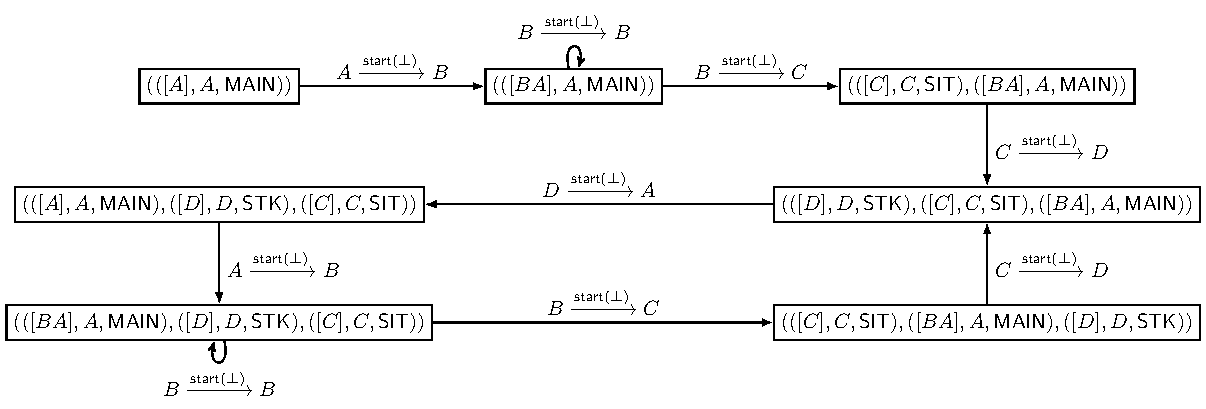
\includegraphics[scale = 0.75]{iff-example.pdf}
        \caption{Configurations reachable from the initial configuration $(([A], A,\mainflag))$ in a $\LMAOAMASS$ $\Mm$}
            %in $\phi$
    % \vspace{-6mm}	
    \label{iff-example}
\end{figure}

    % and $\lmd(D_1) = \lmd(D_2) = \STD$, $\lmd(P_1) = \lmd(P_2) = \STP$, $\lmd(K_1) = \lmd(K_2) = \STK$, $\lmd(T_1) = \lmd(T_2) = \SIT$, and $\aft(D_1) = \aft(P_1) = \aft(K_1) = \aft(T_1) = 1$, $\aft(D_2) = \aft(P_2) = \aft(K_2) = \aft(T_2) = 2$.
\end{example}

From the informal description and the example above, we have already gotten an intuitive understanding of the semantics of $\Mm$. 
To facilitate a precise understanding of the semantics of $\LMAOAMASS$, let us formally define the semantics of $\Mm$ as a transition relation $\xrightarrow{\Mm} $ in the sequel. 

\paragraph{Transition relation.} We define the relation $\xrightarrow{\Mm} $ which comprises the quadruples $(\rho, \tau, \rho') \in \conf_\Mm \times \Delta  \times \conf_\Mm$ 
%$(\rho, \ell) \xrightarrow{\Mm} (\rho', \ell')$ on $\conf_\Mm$ 
to formalise the semantics of $\Mm$. For readability, 
we write $(\rho, \tau, \rho')\in \xrightarrow{\Mm}$  as $\rho \xrightarrow[\tau]{\Mm} \rho'$.
% we write $((\rho,\ell), \tau, (\rho',\ell'))\in \xrightarrow{\Mm}$  as $(\rho,\ell) \xrightarrow[\tau]{\Mm} (\rho',\ell')$.
%Intuitively, $i = 0, 1, 2$ corresponds to the cases that the top task of $\rho$ is absent in $\rho'$, remains to be the top task of $\rho'$, or becomes the task immediately below the top task, of $\rho'$ respectively. 

Let $\rho = ((S_1, A_1, \zeta_1), \cdots, (S_n, A_n, \zeta_n))$ be the current configuration for some $n \ge 1$ and $\topact(\rho) = A$. Moreover, let $S_1 = [A'_1, \cdots, A'_m]$. Evidently, $A = A'_1$.

If $\tau = \back$, then $\rho' = ((S'_1, A_1, \zeta_1), (S_2, A_2, \zeta_2) \cdots, (S_n, A_n, \zeta_n))$ if $m > 1$, where $S'_1 = [A'_2, \cdots, A'_m]$, and $\rho' = ((S_2, A_2, \zeta_2) \cdots, (S_n, A_n, \zeta_n))$ otherwise. 

Then let us consider $\tau = A\xrightarrow{\startactivity(\phi)}B$. 
%\jinlong{put the semantics of $\finishstart$ in Appendix~\ref{app-finishstart-lmaoamss}.}

%Let $\rho = ((S_1, A_1, \zeta_1), \cdots, (S_n, A_n, \zeta_n))$ be the current configuration for some $n \ge 1$ and $\topact(\rho) = A$.

%As the semantics of {\AMASS} are highly complex even if we consider only the semantics of activities separately, hence we will formalize the semantics step by step. Firstly, we consider the case without the intent flag, then we consider the case with only the intent flag, and finally we consider the complete semantics.
%\subsection*{\revision{Case: intent-flag free}}
%In this case, we only consider the launch modes and task affinities, that is, $\phi = \bot$. Launch modes and task affinities are the attributes of an activity, recall that a task is a collection of activities to carry out a certain job, the launch modes are used to define how an activity is associated with the task as Table~\ref{tab-int-lm} shown, and the task affinities are used to define how an activity tends to belong to a particular task. By default, all activities within the same application have the same affinity. Therefore, by default, all activities within the same application tend to be in the same task.

% We consider the subcase $\alpha = \startactivity$ first, the subcase $\alpha = \finishstart$ could be defined according to the former subcase.


\smallskip
\noindent \fbox{$\lmd(B) = \STD$}
	\begin{itemize}
		\item If $\lmd(A) \neq \SIT$, then $\rho'= \push(\rho,B)$.
		%
		\item If $\lmd(A) = \SIT$, then
    		\begin{itemize}
                \item if $\getrealtsk(\rho,B) = S_i$ and $\zeta_i\neq\mainflag$, then $\rho'=\mvtsktop(\rho, i)$,
                \item if $\getrealtsk(\rho,B) = S_i$ and $\zeta_i = \mainflag$, or $\getrealtsk(\rho,B) = *\wedge \gettsk(\rho,B) = S_i$, \\then $\rho'=\push(\mvtsktop(\rho, i),B)$,
    			\item if $\gettsk(\rho, B)=*$, then $\rho'= \newtsk(\rho, B, \STK)$.
    		\end{itemize}
	\end{itemize}

\noindent  \fbox{$\lmd(B) = \STP$}
	\begin{itemize}
		\item  If $\lmd(A) \neq \SIT$, then
        \begin{itemize}
            \item if $A = B$, then $\rho' = \rho$,
            \item otherwise, $\rho' = \push(\rho, B)$.
        \end{itemize}
		%
		\item If $\lmd(A) = \SIT$, then
    		\begin{itemize}
                \item if $\getrealtsk(\rho,B) = S_i$ and $\zeta_i\neq\mainflag$, then $\rho'=\mvtsktop(\rho, i)$,
                \item if $\getrealtsk(\rho,B) = S_i$ and $\zeta_i = \mainflag$, or $\getrealtsk(\rho,B) = *\wedge \gettsk(\rho,B) = S_i$, 
                \begin{itemize}
                    \item if $\topact(S_i) = B$, then $\rho' = \mvacttop(\rho,i)$,
                    \item otherwise $\rho'=\push(\mvtsktop(\rho, i),B)$,
                \end{itemize}
                % then $\rho'=\push(\mvtsktop(\rho, i),B)$,
    			\item if $\gettsk(\rho, B)=*$, then $\rho'= \newtsk(\rho,B, \STK)$.
    		\end{itemize}
	 \end{itemize}
	
\noindent \fbox{$\lmd(B) = \SIT$}
\begin{itemize}
	\item If $\getrealtsk(\rho, B) = S_i$, then $\rho' = \mvtsktop(\rho, i)$.
	\item If $\getrealtsk(\rho, B) = *$, then $\rho' = \newtsk(\rho, B,\SIT)$.
\end{itemize}

\noindent  \fbox{$\lmd(B) = \singletask$}
\begin{itemize}
	\item If $\getrealtsk(\rho, B) = S_i$, or $\getrealtsk(\rho,B) = *\wedge\gettsk(\rho,B) = S_i$ then
	\begin{itemize}
        \item if $B \not \in S_i$, then $\rho' = \push(\mvtsktop(\rho, i), B)$,
        \item if $B \in S_i$, 	then $\rho' =  \clrtop(\mvtsktop(\rho, i), B)$.
	\end{itemize}
\item If $\gettsk(\rho, B) = *$, then $\rho' = \newtsk(\rho, B,\STK)$.
\end{itemize}
From the definition of the semantics, we can see that a new task $([B], B, \STK)$ is created, not only when $\lmd(B) = \STK$, but also when $\lmd(A) = \SIT$ and $\lmd(B) = \STD$.
% \noindent\emph{Case: $\alpha = \finishstart$}

% In this subcase, $A\xrightarrow{\finishstart(\bot)}B$ specifies that $B$ is started followed by the termination of $A$, popped from the task stack. Let $\tau' = A\xrightarrow{\startactivity(\bot)}B$ and $\rho\xrightarrow[\tau']{\Mm}\rho''$ with $\rho''=((S_1',A_1',b_1'),\cdots,(S_{n'}',A_{n'}',b_{n'}'))$.
% \begin{itemize}
%     \item If $A_1\neq A_1'$, it means that the $A_1'$-task is the top task instead of $A_1$-task, hence $A$ is the top activity of $S_2'$, then $\rho' = \rmact(\rho'',2,1)$.
%     \item If $A_1=A_1$, it means that $A_1$-task is still the top task.
%     \begin{itemize}
%         \item if $|S_1|>|S_1'|$, it means that $A$ has popped, then $\rho' = \rho''$,
%         \item if $|S_1|<|S_1'|$, it means that $A$ is the second to top activity of $S_1'$, then $\rho' = \rmact(\rho'',1,2)$,
%         \item if $|S_1|=|S_1'|$, it means that $A$ is the top activity of $S_1'$, then $\rho' = \rmact(\rho'',1,1)$.
%     \end{itemize}
% \end{itemize}

%Finally, let us consider $\tau = A\xrightarrow{\finishstart(\phi)}B$.  
%The semantics of $A\xrightarrow{\finishstart(\phi)}B$ is defined the same as follows: Assume that $\rho \xrightarrow[\tau']{\Mm} \rho''$ where $\tau' = A\xrightarrow{\startactivity(\phi)}B$. Compute the index $(i,j)$ of $A$ in $\rho''$, that is the $j$-th activity of the $i$-th task in $\rho''$ is $A$, then $\rho' = \rmact(\rho'',i,j)$




%%%%%%%%%%%%%% Semantics of IFAOAMASS %%%%%%%%%%%
%%%%%%%%%%%%%% Semantics of IFAOAMASS %%%%%%%%%%%
%%%%%%%%%%%%%% Semantics of IFAOAMASS %%%%%%%%%%%

\smallskip
\noindent {\bf Semantics of $\IFAOAMASS$}.

\smallskip

The intuitions of the intent flags are given in Table~\ref{tab-int-flag}. We would like to warn that although the intuitions of these intent flags may help the readers to get some preliminary idea of their meanings, before diving directly into the formal semantics, they are nonetheless inaccurate, especially when different flags may interfere with each other. 
%, before defining the formal semantics of $\IFAOAMASS$.

\begin{table}[htbp]
\begin{center}
\small
    \begin{tabular}{|m{5.5cm}<{\centering}|m{2cm}<{\centering}|m{6cm}<{\centering}|}
    \hline
    \textbf{Intent Flags} & \textbf{Abbreviation} & \textbf{Intuition} \\
    \hline
	$\rm  FLAG\_ACTIVITY\_SINGLE\_TOP$ & $\stpflag$ & If it is set,  it has the same effect as starting an activity of the $\STP$ launch mode.\\
    \hline
	$\rm FLAG\_ACTIVITY\_CLEAR\_TOP$ & $\ctpflag$ & If it is set,  all the activities above the topmost occurrence of the started activity in the top task will be removed.\\
    \hline
	$\rm FLAG\_ACTIVITY\_REORDER\_TO\_FRONT$ & $\rtfflag$ & If it is set, it will check for the existence of the started activity in the task. If an instance of the activity exists, then the topmost occurrence of this activity will be moved to the top of this task. Otherwise, a new instance of the activity will be pushed into the top task.\\
    \hline
	$\rm FLAG\_ACTIVITY\_NEW\_TASK$ & $\ntkflag$ & If it is set, it will look for an existing task to put the started activity according to the task allocation mechanism. If such a task exists, the task will be moved to the top and a new instance of the activity is pushed to the task, otherwise a new task is created to put this activity.\\
    \hline
	$\rm FLAG\_ACTIVITY\_NEW\_DOCUMENT$ & $\ndmflag$ & If it is set, its behavior is similar to the $\STK$ launch mode, but the task allocation mechanism is slightly different, namely, it will look for an existing task by only using real activities of tasks, but not affinities.\\
    \hline
	$\rm FLAG\_ACTIVITY\_MULTIPLE\_TASK$ & $\mtkflag$ & It is usually used together with $\ntkflag$ or $\ndmflag$. If it is set, then it will always create a new task to put the started activity, no matter whether there already exists a task of the same affinity as this activity.\\
    \hline
	$\rm  FLAG\_ACTIVITY\_CLEAR\_TASK$ & $\ctkflag$ &  It is usually used together with $\ntkflag$ or $\ndmflag$. If it is set, it will remove all the activities in the task and push the started activity to the task.\\
    \hline
	$\rm  FLAG\_ACTIVITY\_NO\_HISTORY$ & $\nohflag$ & If it is set,  when the started activity becomes a non-topmost activity in the future, the activity will be removed.\\
    \hline
	$\rm  FLAG\_ACTIVITY\_PREVIOUS\_IS\_TOP$ & $\pitflag$ & If it is set, then when starting this activity, the activity immediately below the topmost activity will play the role of the topmost activity.\\
    \hline
%	$\rm  FLAG\_ACTIVITY\_RESET\_TASK\_IF\_NEEDED$ & $\rtnflag$ & It is usually used together with $\ntkflag$ or $\ndmflag$. If it is set, the task which has the same affinity with the caller activity will be moved to the top, when the intent flag $\ntkflag$ or $\ndmflag$ is set.\\
%	If set, and this activity is either being started in a new task or bringing to the top an existing task, then it will be launched as the front door of the task.
%    \hline
	$\rm FLAG\_ACTIVITY\_TASK\_ON\_HOME$ & $\tohflag$ & It is usually used together with $\ntkflag$ or $\ndmflag$. If it is set, then only the top task, which is either a newly created task or an existing task moved to the top, is kept, and all the other tasks are removed. \\
    \hline
    \end{tabular}
\end{center}
    \caption{Intuitions of intent flags}
    \label{tab-int-flag}
\end{table}

%\jinlong{omit $\nohflag$ here, and give an intuition of the $\nohflag$, the details defined in Appendix~\ref{app-ifaoamass}.}

To ease the presentation, let us assume that $\phi\models \neg \nohflag$ in $A \xrightarrow{\startactivity(\phi)} B$. The full semantics of $\IFAOAMASS$ where the situation $\phi \models \nohflag$ is taken into consideration can be found in Appendix~~\ref{app-ifaoamass}.


%To define the semantics of $\IFAOAMASS$, we adapt slightly the notion of configurations and add some auxiliary functions and predicates. 
Let $\Mm$ be an $\IFAOAMASS$, namely, $\lmd(A) = \STD$ for each activity $A$.



%It turns out that the flag $\nohflag$ makes the definition of the semantics tedious. For instance, if the current top activity of the top task is started with the flag $\nohflag$, then it should be removed if it is not the top activity of the top task anymore after the application of a transition rule. To ease the understanding, we omit the flag $\nohflag$ first, and give a intuition of the semantics of $\Mm$ with $\nohflag$ later, the details of the formal semantics of $\Mm$ is defined in Appendix~\ref{app-ifaoamass}.
%Moreover we can largely reuse the definition of semantics of the case $\phi\models\neg\tohflag$. 
%In the sequel, $\nohflag$ is ignored first, and we distinguish two subcases, i.e., $\phi \models \neg \tohflag$ and $\phi \models \tohflag$.


To define the semantics of $\Mm$, the concept of configurations is adapted from the definition of configurations for  $\LMAOAMASS$ as follows: 
A configuration of $\Mm$ is 
still encoded as a sequence
% encoded as a pair $(\rho, b)$, where $b \in \{\nohflag, \neg \nohflag\}$ and 
$\rho=(\Omega_1,\cdots,\Omega_n)$ such that for each $i \in [n]$, $\Omega_i = (S_i, A_i, \zeta_i)$, where $S_i \in \act^*$ is a task, $A_i \in \act$ is the real activity of $S_i$, but $\zeta_i \in \{\mainflag, \ntkflag, \ndmflag\}$. Intuitively, 
% $b$ denotes whether the topmost activity is started with $\nohflag$ or not, 
$\ntkflag$ in $\zeta_i$ plays the same role as $\STK$ in $\LMAOAMASS$, and $\ndmflag$ is added for the intent flag $\ndmflag$, moreover, $\SIT$ disappears since in $\IFAOAMASS$, the launch modes of all activities are assumed to be $\STD$.


Then we introduce some additional auxiliary functions and predicates to be used in the formal semantics of $\Mm$.

\paragraph{Auxiliary functions and predicates.} 
Let $\rho = (\Omega_1,\cdots,\Omega_n)$ be a configuration with  $\Omega_i = (S_i, A_i, \zeta_i)$ for each $i\in[n]$, and $S=[B_1,\cdots,B_m]$ be a task. 
% Let $(\rho,b)$ be a configuration with $\rho = (\Omega_1,\cdots,\Omega_n)$ and $\Omega_i = (S_1,A_i,\zeta_i)$ for each $i\in[n]$, and $S=[B_1,\cdots,B_m]$ be a task. 
The following additional auxiliary functions are defined. 
\begin{itemize}
	%	\item $\realact(S) = A$, where $S$ is created by an action $start(A,\Ff)$
    \item $\preact(S) = B_2$ if $m> 1$, $\preact(S) = B_1$ otherwise,
	%	\item.  %, ~\mbox{where}~ S = (\act^*)A$\push

	\item $\preact(\rho) = \preact(\toptsk(\rho))$,
	
	\item $\mvacttop(\rho, B)  =(([B]\cdot S'_1 \cdot S''_1,A_1,\zeta_1), \Omega_2, \cdots, \Omega_n) $, 
        if $S_1=S'_1 \cdot[B]\cdot S''_1$ with $S'_1 \in (\act \setminus \{B\})^*$,

    % \item let $1 \le i \le n$, $S_i = [C_1, \cdots, C_l]$ and $1 \le j \le l$, then $\rmact(\rho,i, j) = (\Omega_1,\cdots,\Omega_{i-1},(S_i',A_i,\zeta_i),\Omega_{i+1},\cdots,\Omega_n)$ if $l>1$, where $S_i' = [C_1,\cdots, C_{j-1}, C_{j+1},\cdots, C_l]$, and $\rmact(\rho,i, j) = (\Omega_1,\cdots,\Omega_{i-1},\Omega_{i+1},\cdots,\Omega_n)$ otherwise,

	%---------------------------------------------------------------------------------------------------------------	
	%
	%-------------------------------------------------------------------------------------------------
\end{itemize}
Intuitively, $\preact(S)$ and $\preact(\rho)$ are used for defining the semantics of $\pitflag$, and $\mvacttop(\rho, B)$ is used for defining the semantics of $\rtfflag$.
% and $\rmact(\rho,i, j)$ is used for defining the semantics of $\nohflag$. 
Moreover, the function $\gettsk$ is adapted by replacing $\STK$ with $\ntkflag$: $\gettsk(\rho, B) = S_i$ such that $i \in [n]$ is the \emph{minimum} index satisfying $\aft(A_i)=\aft(B)$ and $\zeta_i \in \{\mainflag,\ntkflag\}$, if such an index $i$ exists; $\gettsk(\rho, B) = *$ otherwise.


Before the formal definition, let us use the following example to illustrate the semantics of the $\IFAOAMASS$. 
%
\begin{example}\label{exam:ifo-amass}
    Let $\Mm = (\act, A, \frag, \lmd, \aft, \vgr, \Delta)$ be an $\IFAOAMASS$, where $\act = \{A,B,C,D,E,F,G\}$, and for each $A' \in\act$, $\lmd(A') = \STD$ and $\aft(A') = 1$.
    Moreover, $\Delta = \{\back\} \cup \{\tau_i \mid 1 \le i \le 9\}$, where 
    % $\rho_0 = (([D_1],D_1,1))$, and\\
        $\tau_1 = A\xrightarrow{\startactivity(\ctpflag)}B$,
        $\tau_2 = B\xrightarrow{\startactivity(\bot)}C$,
        $\tau_3 = B\xrightarrow{\startactivity(\ntkflag\wedge\mtkflag)}D$,
        $\tau_4 = B\xrightarrow{\startactivity(\ndmflag)}F$,
        $\tau_5 = C\xrightarrow{\startactivity(\ntkflag)}A$,
        $\tau_6 = D\xrightarrow{\startactivity(\stpflag)}D$,
        $\tau_7 = D\xrightarrow{\startactivity(\rtfflag)}E$,
        $\tau_8 = E\xrightarrow{\startactivity(\stpflag\wedge\pitflag)}D$,
        $\tau_9 = E\xrightarrow{\startactivity(\ntkflag\wedge\ctkflag)}F$.
%        $\tau_{10} = F\xrightarrow{\startactivity(\ndmflag)}G$.

        The $\xrightarrow{\Mm}$ relation on the set of configurations that are reachable from the initial configuration $(([A], A, \mainflag))$ is illustrated in Figure~\ref{ifo-example}. 
%
    \begin{figure}[htbp]
        % \vspace{-3mm}
            \centering
            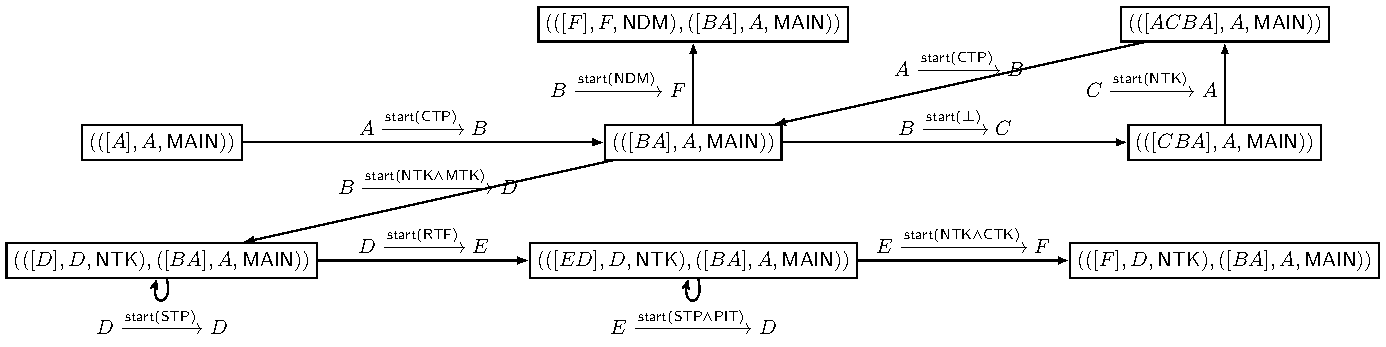
\includegraphics[scale = 0.63]{ifo-example.pdf}
        \caption{Configurations that are reachable from the initial configuration $(([A], A, \mainflag))$ in $\Mm$}
                %in $\phi$
        % \vspace{-6mm}	
        \label{ifo-example}
    \end{figure}
    
For instance,
        \begin{itemize}
        \item from the configuration $(([A], A, \mainflag))$, after executing the transition rule $A \xrightarrow{\startactivity(\ctpflag)} B$, because $\phi \models \neg \ntkflag \wedge \neg \ndmflag$, $B$ does not occur in the top task $[A]$, we have $\rho' = \push((([A], A, \mainflag)), B) = (([BA], A, \mainflag))$, 
		% moreover, $b' = \neg \nohflag$ since $\phi \not \models \nohflag$,
        %
        \item from the configuration $(([ACBA], A, \mainflag))$, after executing $A \xrightarrow{\startactivity(\ctpflag)} B$, because $\phi \models \neg \ntkflag \wedge \neg \ndmflag$, $B$ occurs in the top task $[ACBA]$, we have $\rho' = \clrtop((([ACBA], A, \mainflag)), B) = (([BA], A, \mainflag))$, 
		% moreover, $b' = \neg \nohflag$ since $\phi \not \models \nohflag$, 
 %resulting to the configuration $((([BA], A, \mainflag)),\neg \nohflag)$,
        %
	\item from the configuration $(([BA], A, \mainflag))$, after executing $B\xrightarrow{\startactivity(\bot)}C$, because $\phi\models\neg\ntkflag\wedge\neg\ndmflag\wedge\neg\ctpflag\wedge\neg\rtfflag\wedge\neg\stpflag$,and we have $\rho' = \push((([BA], A, \mainflag)), C) = (([CBA], A, \mainflag))$, 
	% moreover, $b' = \neg \nohflag$ since $\phi \not \models \nohflag$,
	%
	\item from the configuration $(([BA], A, \mainflag))$, after executing $B\xrightarrow{\startactivity(\ndmflag)}F$, because $\phi \models \ndmflag\wedge\neg\mtkflag$, $\getrealtsk(\rho,F) = *$,  we have 
	$\rho' = \newtsk((([BA], A, \mainflag)), F, \ndmflag) = (([F], F, \ndmflag),([BA], A, \mainflag))$, 
	% moreover, $b' = \nohflag$ since $\phi \models \nohflag$,
	%
		\item from the configuration $(([BA], A, \mainflag))$, after executing $B\xrightarrow{\startactivity(\ntkflag\wedge\mtkflag)}D$, because $\phi\models\ntkflag\wedge\neg\ndmflag\wedge\mtkflag$, we have 
		$$\rho' = \newtsk((([BA], A, \mainflag)), D, \ntkflag) = (([D],D,\ntkflag),([BA], A, \mainflag)),$$ 
	% moreover, $b' = \neg \nohflag$ since $\phi \not \models \nohflag$,
        %
        \item from the configuration $(([CBA], A, \mainflag))$, after executing $C \xrightarrow{\startactivity(\ntkflag)} A$, because 
        $\phi\models\ntkflag\wedge\neg\ndmflag\wedge\neg\mtkflag\wedge\neg\ctpflag\wedge\neg\rtfflag\wedge\neg\stpflag$, $\getrealtsk(\rho,A) = S_1$, $\zeta_1 = \mainflag$, we have 
		$$\rho' = \push((([CBA], A, \mainflag)), A) = (([ACBA], A, \mainflag)),$$
		%  moreover, $b' = \neg \nohflag$ since $\phi \not \models \nohflag$,
        %
        \item from the configuration $(([D],D,\ntkflag),([BA], A, \mainflag))$,  after executing  $D \xrightarrow{\startactivity(\stpflag)} D$, because $\phi \models \neg \ntkflag \wedge \neg \ndmflag\wedge\neg\ctpflag\wedge\neg\rtfflag\wedge\stpflag$ and $D$ is the top activity of the top task $[D]$, we have $\rho' = \rho$,
        %
        \item from the configuration $(([D],D,\ntkflag),([BA], A, \mainflag))$, after executing $D \xrightarrow{\startactivity(\rtfflag)} E$, because $\phi \models \neg \ntkflag \wedge \neg \ndmflag\wedge\neg\ctpflag\wedge\rtfflag$ and $E$ dose not occur in the top task $[D]$, we have 
		$$\rho' = \push((([D],D,\ntkflag),([BA], A, \mainflag)), E) = (([ED],D,\ntkflag),([BA], A, \mainflag)),$$
		% moreover, $b' = \neg \nohflag$ since $\phi \not \models \nohflag$,
        %
        \item from the configuration $(([ED],D,\ntkflag),([BA], A, \mainflag))$, after executing $E \xrightarrow{\startactivity(\stpflag\wedge\pitflag)} D$, because $\phi \models \neg \ntkflag \wedge \neg \ndmflag\wedge\neg\ctpflag\wedge\neg\rtfflag\wedge\stpflag\wedge\pitflag$ and $D = \preact([ED])$, we have $\rho' = \rho$, 
        %
        \item from the configuration $(([ED],D,\ntkflag),([BA], A, \mainflag))$, after executing $E \xrightarrow{\startactivity(\ntkflag\wedge\ctkflag)} F$,  because $\phi \models \ntkflag \wedge \neg \ndmflag\wedge\neg\mtkflag\wedge\ctkflag$, $\getrealtsk(\rho,F) = *$ and $\gettsk(\rho,F) = S_1$, we have 
		$$\rho' = \clrtsk((([ED],D,\ntkflag),([BA], A, \mainflag)), F) = (([F],D,\ntkflag),([BA], A, \mainflag)),$$
		%  moreover, $b' = \neg \nohflag$ since $\phi \not \models \nohflag$,
        %
\end{itemize}
\hide{
        \begin{itemize}
        \item from the configuration $((([A], A, \mainflag)), \neg \nohflag)$, after executing the transition rule $A \xrightarrow{\startactivity(\ctpflag)} B$, because $\phi \models \neg \ntkflag \wedge \neg \ndmflag$, $B$ does not occur in the top task $[A]$, $b = \neg \nohflag$, we have $\rho' = \push((([A], A, \mainflag)), B) = (([BA], A, \mainflag))$, moreover, $b' = \neg \nohflag$ since $\phi \not \models \nohflag$,
        %
        \item from the configuration $((([ACBA], A, \mainflag)), \neg \nohflag)$, after executing $A \xrightarrow{\startactivity(\ctpflag)} B$, because $\phi \models \neg \ntkflag \wedge \neg \ndmflag$, $B$ occurs in the top task $[ACBA]$, $b = \neg \nohflag$, we have $\rho' = \clrtop((([ACBA], A, \mainflag)), B) = (([BA], A, \mainflag))$, moreover, $b' = \neg \nohflag$ since $\phi \not \models \nohflag$, 
 %resulting to the configuration $((([BA], A, \mainflag)),\neg \nohflag)$,
        %
	\item from the configuration $((([BA], A, \mainflag)),\neg \nohflag)$, after executing $B\xrightarrow{\startactivity(\bot)}C$, because $\phi\models\neg\ntkflag\wedge\neg\ndmflag\wedge\neg\ctpflag\wedge\neg\rtfflag\wedge\neg\stpflag$,and $b=\neg\nohflag$, we have $\rho' = \push((([BA], A, \mainflag)), C) = (([CBA], A, \mainflag))$, moreover, $b' = \neg \nohflag$ since $\phi \not \models \nohflag$,
	%
	\item from the configuration $((([BA], A, \mainflag)),\neg \nohflag)$, afte executing $B\xrightarrow{\startactivity(\nohflag)}F$, because $\phi\models\neg\ntkflag\wedge\neg\ndmflag\wedge\neg\ctpflag\wedge\neg\rtfflag\wedge\neg\stpflag$, and $b = \neg\nohflag$, we have $\rho' = \push((([BA], A, \mainflag)), F) = (([FBA], A, \mainflag))$, moreover, $b' = \nohflag$ since $\phi \models \nohflag$,
	%
		\item from the configuration $((([BA], A, \mainflag)),\neg \nohflag)$, after executing $B\xrightarrow{\startactivity(\ntkflag\wedge\mtkflag)}D$, because $\phi\models\ntkflag\wedge\neg\ndmflag\wedge\mtkflag$ and $b = \neg\nohflag$, we have 
		$$\rho' = \newtsk((([BA], A, \mainflag)), D, \ntkflag) = (([D],D,\ntkflag),([BA], A, \mainflag)),$$ 
	moreover, $b' = \neg \nohflag$ since $\phi \not \models \nohflag$,
        %
        \item from the configuration $((([CBA], A, \mainflag)), \neg \nohflag)$, after executing $C \xrightarrow{\startactivity(\ntkflag)} A$, because $\phi\models\ntkflag\wedge\neg\ndmflag\wedge\neg\mtkflag\wedge\neg\ctpflag\wedge\neg\rtfflag\wedge\neg\stpflag$, $\getrealtsk(\rho,A) = S_1$, $\zeta_1 = \mainflag$, and $b = \neg \nohflag$, we have 
		$$\rho' = \push((([CBA], A, \mainflag)), A) = (([ACBA], A, \mainflag)),$$
		 moreover, $b' = \neg \nohflag$ since $\phi \not \models \nohflag$,
        %
        \item from the configuration $((([D],D,\ntkflag),([BA], A, \mainflag)),\neg\nohflag)$,  after executing  $D \xrightarrow{\startactivity(\stpflag)} D$, because $\phi \models \neg \ntkflag \wedge \neg \ndmflag\wedge\neg\ctpflag\wedge\neg\rtfflag\wedge\stpflag$ and $D$ is the top activity of the top task $[D]$, we have $(\rho',b') = (\rho,b)$,
        %
        \item from the configuration $((([D],D,\ntkflag),([BA], A, \mainflag)),\neg\nohflag)$, after executing $D \xrightarrow{\startactivity(\rtfflag)} E$, because $\phi \models \neg \ntkflag \wedge \neg \ndmflag\wedge\neg\ctpflag\wedge\rtfflag$ and $E$ dose not occur in the top task $[D]$, we have 
		$$\rho' = \push((([D],D,\ntkflag),([BA], A, \mainflag)), E) = (([ED],D,\ntkflag),([BA], A, \mainflag)),$$
		moreover, $b' = \neg \nohflag$ since $\phi \not \models \nohflag$,
        %
        \item from the configuration $((([ED],D,\ntkflag),([BA], A, \mainflag)),\neg\nohflag)$, after executing $E \xrightarrow{\startactivity(\stpflag\wedge\pitflag)} D$, because $\phi \models \neg \ntkflag \wedge \neg \ndmflag\wedge\neg\ctpflag\wedge\neg\rtfflag\wedge\stpflag\wedge\pitflag$ and $D = \preact([ED])$, we have $(\rho',b') = (\rho,b)$, 
        %
        \item from the configuration $((([ED],D,\ntkflag),([BA], A, \mainflag)),\neg\nohflag)$, after executing $E \xrightarrow{\startactivity(\ntkflag\wedge\ctkflag)} G$,  because $\phi \models \ntkflag \wedge \neg \ndmflag\wedge\neg\mtkflag\wedge\ctkflag$, $\getrealtsk(\rho,G) = *$ and $\gettsk(\rho,G) = S_1$, we have 
		$$\rho' = \clrtsk((([ED],D,\ntkflag),([BA], A, \mainflag)), G) = (([G],D,\ntkflag),([BA], A, \mainflag)),$$
		 moreover, $b' = \neg \nohflag$ since $\phi \not \models \nohflag$,
        %
        \item from the configuration $((([FBA], A, \mainflag)),\nohflag)$, after executing $F \xrightarrow{\startactivity(\ndmflag)} G$, because $\phi \models \ndmflag\wedge\neg\mtkflag\wedge\ctkflag$, $\getrealtsk(\rho,G) = *$, and $b = \nohflag$,  we have 
		$$\rho' = \rmact(\newtsk((([FBA], A, \mainflag)),G,\ndmflag),2,1) = (([G],G,\ndmflag),([BA], A, \mainflag)),$$ 
		moreover, $b' = \neg \nohflag$ since $\phi \not \models \nohflag$.
\end{itemize}
}
%    
\end{example}

The aforementioned informal description of intent flags and the example %enable us to 
provide the intuition of %understand 
the semantics of $\IFAOAMASS$. 
In the sequel, we formally define the semantics of $\Mm$ as a transition relation $\rho \xrightarrow[\tau]{\Mm} \rho'$ with $\tau = A \xrightarrow{\startactivity(\phi)} B$.

Let us assume $\phi \models \neg \tohflag$ first.

\smallskip

%We are ready to define the semantics of $\IFAOAMASS$. 
%The semantics of the transition rule $\back$ is similar to that of $\LMAOAMASS$. 
%Let us focus on the transition rules $A \xrightarrow{\startactivity(\phi)} B$. 

%\jinlong{omit $\nohflag$ here, and give an intuition of the $\nohflag$, the details defined in Appendix~\ref{app-ifaoamass}.}

%It turns out that the flag $\nohflag$ makes the definition of the semantics tedious. For instance, if the current top activity of the top task is started with the flag $\nohflag$, then it should be removed if it is not the top activity of the top task anymore after the application of a transition rule. To ease the understanding, we omit the flag $\nohflag$ first, and give a intuition of the semantics of $\Mm$ with $\nohflag$ later, the details of the formal semantics of $\Mm$ is defined in Appendix~\ref{app-ifaoamass}.
%Moreover we can largely reuse the definition of semantics of the case $\phi\models\neg\tohflag$. 
% Therefore, we assume that $\phi \models \neg \tohflag \wedge \neg \nohflag$ and $b = \neg \nohflag$ first. 
% in the sequel, we present the full semantics for the situation $b = \neg \nohflag$, but only illustrates the semantics partially for the situation $b =  \nohflag$ and delegate the full semantics to Appendix~\ref{app-sem-ifaoamass}.
% We first assume that $\phi \models \neg \tohflag \wedge \neg \nohflag$. We will consider $\phi \models \tohflag$ and $\phi \models \nohflag$ in the end. 
%In the sequel, $\nohflag$ is ignored first, and we distinguish two subcases, i.e., $\phi \models \neg \tohflag$ and $\phi \models \tohflag$.

%Let us define the semantics of $\Mm$ by a relation 
% $\rho \xrightarrow[\Mm]{\startactivity(\phi)} \rho'$ with $\phi \models \neg \tohflag \wedge \neg \nohflag$.
%$\rho \xrightarrow[\tau]{\Mm} \rho'$ with $\tau = A \xrightarrow{\startactivity(\phi)} B$.
%Let us consider the subcase $\phi \models \neg \tohflag$ first.

\noindent \fbox{$\phi \models \neg \ntkflag\wedge\neg\ndmflag$}
	\begin{itemize}
		\item If $\phi \models \ctpflag$ and $B \in \toptsk(\rho)$, then $\rho' = \clrtop(\rho, B)$.
		\item If $\phi \models \ctpflag$ and $B \notin \toptsk(\rho)$, then $\rho' = \push(\rho, B)$.
		\item If $\phi \models \neg \ctpflag$, then
		\begin{itemize}
			\item if $\phi \models \rtfflag$ and $B \in \toptsk(\rho)$, then $\rho'= \mvacttop(\rho, B)$, 
			\item if $\phi \models \rtfflag$ and $B \notin \toptsk(\rho)$, then $\rho' = \push(\rho, B)$, 
			\item if $\phi \models \neg \rtfflag$, then
			\begin{itemize}
				\item if $\phi \models \stpflag$ and $\topact(\rho) = B$ or $\phi \models \stpflag\wedge\pitflag$ and $\preact(\rho) = B$, then $\rho' = \rho$,
				\item otherwise, $\rho' = \push(\rho, B)$.
			\end{itemize}
		\end{itemize}
\end{itemize}

% 
\noindent \fbox{$\phi \models \ndmflag$}

\begin{itemize}
    \item If $\phi \models \mtkflag$, then $\rho'=\newtsk(\rho, B, \ndmflag)$.
    %
    \item If $\phi \models \neg \mtkflag$, then
   \begin{itemize}
        \item if $\getrealtsk(\rho, B) = S_i$, then
		\begin{itemize}
			\item if $\phi \models \ctkflag$, then $\rho' = \clrtsk(\mvtsktop(\rho, i), B)$,
			\item if $\phi \models \neg \ctkflag$, then
			\begin{itemize}
				\item if $B\in S_i$, then $\rho' = \clrtop(\mvtsktop(\rho, i), B)$,
				\item if $B\notin S_i$, then $\rho' = \push(\mvtsktop(\rho, i), B)$,
			\end{itemize}
		\end{itemize}
        \item if $\getrealtsk(\rho, B) = *$, then $\rho' = \newtsk(\rho, B, \ndmflag)$.
	\end{itemize}
\end{itemize}

% 
\smallskip
\noindent \fbox{$\phi \models \ntkflag \wedge \neg \ndmflag$}

\begin{itemize}
\item If $\phi \models \mtkflag$,  then $\rho' = \newtsk(\rho, B, \ntkflag)$.
%
\item If $\phi \models \neg \mtkflag$,  then
	\begin{itemize}
        \item if $\getrealtsk(\rho, B) = S_i$ or $\getrealtsk(\rho,B) = * \wedge\gettsk(\rho,B) = S_i$, then
		\begin{itemize}
			\item if $\phi \models \ctkflag$, then $\rho'=\clrtsk(\mvtsktop(\rho, i), B)$,
			\item if $\phi \models \neg \ctkflag$, then
			\begin{itemize}
				\item if $\phi \models \ctpflag$ and $B \in S_i$, then 
				$\rho'=\clrtop(\mvtsktop(\rho, i), B)$,
				\item if $\phi \models \ctpflag$ and $B \notin S_i$, then 
				$\rho'=\push(\mvtsktop(\rho, i), B)$,
				\item if $\phi \models \neg \ctpflag$, then
				\begin{itemize}
					\item if $\phi \models \rtfflag$ and $B \in S_i$, then
				$\rho'=\mvacttop(\mvtsktop(\rho, i), B)$,
					\item if $\phi \models \rtfflag$ and $B \notin S_i$, then
				$\rho'=\push(\mvtsktop(\rho, i), B)$,
					\item if $\phi \models \neg \rtfflag$, then
					\begin{itemize}
						\item if $\getrealtsk(\rho, B) = S_i$ and $\zeta_i \neq \mainflag$, 
						then $\rho' = \mvtsktop(\rho, i)$,
						\item otherwise, 
						\begin{itemize}
							\item if $\phi \models \stpflag$ and $\topact(S_i) = B$, or $\phi \models \stpflag \wedge \pitflag$ and $i = 1$ and $\preact(S_1) = B$, then $\rho' = \mvtsktop(\rho, i)$,
							\item otherwise, $\rho'=\push(\mvtsktop(\rho, i), B)$,
						\end{itemize}
					\end{itemize}
				\end{itemize}
			\end{itemize}
		\end{itemize}
	    %
	\item if $\gettsk(\rho, B) = *$, then $\rho' = \newtsk(\rho, B, \ntkflag)$.
	\end{itemize}
\end{itemize}

Finally we consider the situation $\phi \models \tohflag$.
% and $\nohflag$ is still ignored.
Let $\phi'$ be obtained from $\phi$ by replacing $\tohflag$ with $\neg \tohflag$. Moreover, 
suppose $\rho \xrightarrow [\tau']{\Mm} \rho'$, where $\tau' = A \xrightarrow{\startactivity(\phi')} B$ and $\rho' = (\Omega_1, \cdots, \Omega_{n})$. 
% suppose $(\rho, b) \xrightarrow [\startactivity(\phi')]{\Mm} (\rho', b')$, where $\rho' = (\Omega_1, \cdots, \Omega_{n})$. 
Then
\begin{itemize}
\item if $\phi \models \ntkflag \vee \ndmflag$, then let $\rho'' = (\Omega_1)$ and we have $\rho \xrightarrow [\tau]{\Mm} \rho''$,
%
\item otherwise, $\rho \xrightarrow [\tau]{\Mm} \rho'$.
\end{itemize}


%%%%%%%%%%%%%%%%%%%%%move to the appendix%%%%%%%%%%%%%%%%%%%
%%%%%%%%%%%%%%%%%%%%%move to the appendix%%%%%%%%%%%%%%%%%%%
\hide{
At last, let us consider the semantics of $\Mm$ with $\nohflag$. Firstly, we need adapt the concept of configurations as follows:
A configuration of $\Mm$ is encoded as a pair $(\rho, b)$, where $b \in \{\nohflag, \neg \nohflag\}$. Intuitively, $b$ denotes whether the topmost activity is started with $\nohflag$ or not.

% Now let us define the semantics of $\Mm$ by a relation $(\rho,b)\xrightarrow[\tau]{\Mm}(\rho',b')$ with $\tau = A\xrightarrow{\startactivity(\phi)}B$.
% Let $\phi'$ be obtained from $\phi$ by replacing $\nohflag$ with $\neg \nohflag$. Moreover, 
Suppose $\rho \xrightarrow [\tau]{\Mm} \rho'$.
Intuitively, $(\rho,b)\xrightarrow[\tau]{\Mm} (\rho'', b')$ is defined as follows:
\begin{itemize}
	\item If $b = \neg\nohflag$, then $\rho'' = \rho'$ 
	\begin{itemize}
		\item if $\phi \models \nohflag$, and the top activity of the top task in $\rho'$ is a fresh activity, then $b' = \nohflag$,
		\item otherwise, $b' = \neg \nohflag$.
	\end{itemize}
	\item If $b = \nohflag$, then
	\begin{itemize}
		\item if the top activity of the top task in $\rho$ is still the top activity of the top task in $\rho''$, then $\rho'' = \rho'$ and $b' = b$.
		\item otherwise, $\rho''$ is obtained from $\rho'$ by removing the original top activity of the top task in $\rho$, moreover,
		\begin{itemize}
			\item if $\phi \models \nohflag$, and the top activity of the top task in $\rho'$ is a fresh activity, then $b' = \nohflag$,
			\item otherwise, $b' = \neg \nohflag$.
		\end{itemize}
	\end{itemize}
\end{itemize}

% \noindent\emph{Case: $\alpha = \finishstart$}

% Similarly, let $\tau' = A\xrightarrow{\startactivity(\phi)}B$ and $\rho\xrightarrow[\tau']{\Mm}\rho''$ with $\rho''=((S_1',A_1',b_1'),\cdots,(S_{n'}',A_{n'}',b_{n'}'))$.
% \begin{itemize}
%     \item If $A_1\neq A_1'$, it means that the $A_1'$-task is the top task instead of $A_1$-task, hence $A$ is the top activity of $S_2'$, then $\rho' = \rmact(\rho'',2,1)$.
%     \item If $A_1=A_1$, it means that $A_1$-task is still the top task.
%     \begin{itemize}
%         \item if $|S_1|>|S_1'|$, it means that $A$ has popped, then $\rho' = \rho''$,
%         \item if $|S_1|<|S_1'|$, it means that $A$ is the second to top activity of $S_1'$, then $\rho' = \rmact(\rho'',1,2)$,
%         \item if $|S_1|=|S_1'|$, it means that $A$ is the top activity of $S_1'$, then $\rho' = \rmact(\rho'',1,1)$.
%     \end{itemize}
% \end{itemize}

Finally, let us consider the transition rules $A \xrightarrow{\finishstart(\phi)} B$. 
Intuitively, for a configuration $(\rho, b)$, $A \xrightarrow{\finishstart(\phi)} B$ will first start the activity $B$ with the intent flags specified by $\phi$,  then remove the original top activity $A$.
The definition of the semantics of $A \xrightarrow{\finishstart(\phi)} B$ is somehow similar to the semantics of $A \xrightarrow{\startactivity(\phi)} B$ on $(\rho, b)$ with $b = \nohflag$. The difference is that $A$ will always be removed for $A \xrightarrow{\finishstart(\phi)} B$, while this is not the case for $A \xrightarrow{\startactivity(\phi)} B$ and $b = \nohflag$. 
Since the formal semantics of $A \xrightarrow{\finishstart(\phi)} B$ is tedious, we omit it here and put it in Appendix~\ref{app-ifaoamass}. 
}
%%%%%%%%%%%%%%%%%%%%%move to the appendix%%%%%%%%%%%%%%%%%%%
%%%%%%%%%%%%%%%%%%%%%move to the appendix%%%%%%%%%%%%%%%%%%%


%The behavior $A \xrightarrow{\finishstart(\phi)} B$ is similar to $A \xrightarrow{\startactivity(\phi)} B$ and $b = \nohflag$. The difference is that $A$ will be terminated only if when $A$ is not the topmost activity of top task.

%The semantics of the transition rules $A \xrightarrow{\finishstart(\phi)} B$ is adapted from that for $A \xrightarrow{\startactivity(\phi)} B$ as follows:
%\begin{itemize}
%	\item remove the item and sub-items for the constraint $b = \neg\nohflag$,
%	\item replace $\rho' = \rho, b' = b$ with $\rho = \rmact(\rho, 1, 1), b' = \neg\nohflag$ for each item which contains $\rho' = \rho, b' = b$.
%\end{itemize}


By a retrospect of the aforementioned formal semantics, we can discover that the intent flags %are not independent of each other and they 
may interfere with each other. We summarize their dependencies as follows. 

\paragraph{Dependencies of intent flags.}
%Intuitively, for a transition $A\xrightarrow{\alpha(\phi)}B$, the intent flags in $\phi$ may depend on each other. 
The dependencies of intent flags can exhibit in the following two forms: (1) $n$ \emph{subsumes} $n'$, i.e., $n'$ is ignored if $n$ co-occurs with $n'$, and the ``subsume'' relations are transitive, (2) $n$ \emph{enables} $n'$, i.e., $n'$ takes effect if $n$ co-occurs with $n'$. The dependencies among the intent flags are summarized in Figure~\ref{fig-amass-depend}, where the solid lines represent the ``subsume'' relation, the dashed lines represent  the ``enable'' relation.
\begin{figure}[htbp]
    % \vspace{-3mm}
        \centering
        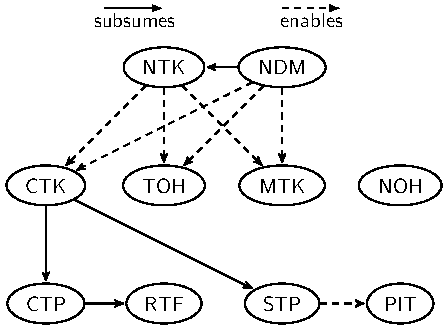
\includegraphics[scale = 0.7]{ifo-amass-dependency.pdf}
        \caption{Dependency graph of intent flags.}
            %in $\phi$
    % \vspace{-6mm}	
    \label{fig-amass-depend}
\end{figure}
\smallskip


\hide{
\smallskip
\noindent \fbox{$\phi \models \neg \ntkflag\wedge\neg\ndmflag$}
	\begin{itemize}
		\item If $\phi \models \ctpflag$ and $B \in \toptsk(\rho)$, then 
		\begin{itemize}
			\item if $\topact(\rho) \neq B$, then $\rho' = \clrtop(\rho, B)$, moreover, 
			\begin{itemize}
			\item if $\phi \models \neg \stpflag$, then $b' = \nohflag$ iff $\phi \models \nohflag$, 
			\item otherwise, $b' = \neg \nohflag$,
			\end{itemize}
			\item if $\topact(\rho) = B$, then $\rho' = \rho$, moreover,
			% $\rho' = \rho$, moreover,
			\begin{itemize}
			 	\item if $\phi \models \neg \stpflag$, then $b' = \nohflag$ iff $\phi \models \nohflag$, 
				\item otherwise, $b' = b$,
			\end{itemize}
		\end{itemize}
		\item If $\phi \models \ctpflag$ and $B \notin \toptsk(\rho)$, then $b' = \nohflag$ iff $\phi \models \nohflag$, moreover,
		\begin{itemize}
			\item if $b = \neg \nohflag$, then $\rho' = \push(\rho, B)$, 
			\item otherwise, $\rho' = \rmact( \push(\rho, B), 1, 2)$. 
		\end{itemize}
		\item If $\phi \models \neg \ctpflag$, then
		\begin{itemize}
			\item if $\phi \models \rtfflag$ and $B \in \toptsk(\rho)$, then
			\begin{itemize}
				\item if $\topact(\rho) \neq B$, then $b' = \neg \nohflag$, moreover, 
				\begin{itemize}
					\item if $b = \neg \nohflag$, then $\rho'= \mvacttop(\rho, B)$, 
					\item otherwise, $\rho' = \rmact(\mvacttop(\rho, B), 1, 2)$, 
				\end{itemize}
				\item if $\topact(\rho) = B$, then $\rho' = \rho$ and $b' = b$,
			\end{itemize}
			\item if $\phi \models \rtfflag$ and $B \notin \toptsk(\rho)$, then $b' = \nohflag$ iff $\phi \models \nohflag$, moreover,
			\begin{itemize}
				\item if $b = \neg \nohflag$, then $\rho' = \push(\rho, B)$, 
				\item otherwise, $\rho' = \rmact( \push(\rho, B), 1, 2)$. 
			\end{itemize}
			\item If $\phi \models \neg \rtfflag$, then
			\begin{itemize}
				\item if $\phi \models \stpflag$ and $\topact(\rho) = B$ or $\phi \models \stpflag\wedge\pitflag$ and $\preact(\rho) = B$, then $\rho' = \rho$ and $b' = b$,
				\item otherwise, $b' = \nohflag$ iff $\phi \models \nohflag$, moreover,
				\begin{itemize}
					\item if $b = \neg \nohflag$, then $\rho' = \push(\rho, B)$, 
					\item otherwise, $\rho' = \rmact( \push(\rho, B), 1, 2)$. 
				\end{itemize}
			\end{itemize}
		\end{itemize}
\end{itemize}

\smallskip
\noindent \fbox{$\phi \models \ndmflag$}

\begin{itemize}
    \item If $\phi \models \mtkflag$, then $b' = \nohflag$ iff $\phi  \models \nohflag$, 
    \begin{itemize}
    	\item if $b = \neg \nohflag$, then $\rho'=\newtsk(\rho, B, \ndmflag)$, 
	\item otherwise, $\rho'= \rmact(\newtsk(\rho, B, \ndmflag), 2, 1)$.
    \end{itemize}
    %
    \item If $\phi \models \neg \mtkflag$, then
   \begin{itemize}
        \item if $\getrealtsk(\rho, B) = S_i$, then
	\begin{itemize}
		\item if $i \neq 1$, then
        			\begin{itemize}
            			\item if $\phi \models \neg \ctkflag$, then 
				\begin{itemize}
					\item if $B \not \in S_i$, then $b' = \nohflag$ iff $\phi  \models \nohflag$, moreover, 
					\begin{itemize}
						\item if $b = \neg \nohflag$, then $\rho' = \push(\mvtsktop(\rho, i), B)$, 
						\item otherwise, $\rho' = \rmact(\push(\mvtsktop(\rho, i), B), 2, 1)$, 
					\end{itemize}
					\item otherwise, $b' = \neg \nohflag$,
					% \begin{itemize}
					% 	\item if $\phi \models \neg \stpflag$, then $b' = \nohflag$ iff $\phi  \models \nohflag$, 
					% 	\item otherwise, $b' = \neg \nohflag$, 
					% \end{itemize}
					moreover, 
					\begin{itemize}
						\item if $b = \neg \nohflag$, then $\rho'=\clrtop(\mvtsktop(\rho, i), B)$, 
						\item otherwise,  $\rho'= \rmact(\clrtop(\mvtsktop(\rho, i), B), 2, 1)$, 
					\end{itemize}
				\end{itemize}
            			\item if $\phi \models \ctkflag$, then $b' = \nohflag$ iff $\phi  \models \nohflag$, moreover, 
				\begin{itemize}
						\item if $b = \neg \nohflag$, then $\rho'=\clrtsk(\mvtsktop(\rho, i), B)$, 
						\item otherwise,  $\rho'= \rmact(\clrtsk(\mvtsktop(\rho, i), B), 2, 1)$, 
				\end{itemize}
        			\end{itemize}
		\item otherwise ($i = 1$), 
        			\begin{itemize}
            			\item if $\phi \models \neg \ctkflag$, then 
            			\begin{itemize}
					\item if $B \not \in S_1$, then $b' = \nohflag$ iff $\phi  \models \nohflag$, moreover, 
					\begin{itemize}
						\item if $b = \neg \nohflag$, then $\rho'=\push(\rho, B)$,
						\item otherwise, $\rho' = \rmact(\push(\rho, B), 1, 2)$,  
					\end{itemize}
            				\item if $B \in S_1$ and $\topact(S_1) \neq B$, then $\rho'= \clrtop(\rho, B)$ and $b' = \neg\nohflag$,
					% \begin{itemize}
					% 	\item if $\phi \models \stpflag$, then $b' = \neg \nohflag$, 
					% 	\item otherwise, $b' = \nohflag$ iff $\phi  \models \nohflag$,
					% \end{itemize}
					\item if $B \in S_1$ and $\topact(S_1) = B$ (this implies $A = B$), then $\rho' = \rho$ and $b' = b$,
			 	\end{itemize}
            			\item if $\phi \models \ctkflag$, then $\rho'= \clrtsk(\rho, B)$, and $b' = \nohflag$ iff $\phi  \models \nohflag$, 
				% \begin{itemize}
				% 	\item if $\phi \models \stpflag$, then $b' = \neg \nohflag$, moreover, 
				% 	\begin{itemize}
				% 		\item if $B \not \in S_1$, then 
				% 	\end{itemize}
				% 	\item otherwise, $b' = \nohflag$	iff $\phi  \models \nohflag$, 		
				% \end{itemize}
            	% 		\begin{itemize}
				% 	\item if $B \not \in S_1$, then $b' = \nohflag$ iff $\phi  \models \nohflag$, moreover, 
				% 	\begin{itemize}
				% 		\item if $b = \neg \nohflag$, then $\rho' = \push(\rho, B)$,
				% 		\item otherwise, $\rho' = \rmact(\push(\rho, B), 1, 2)$, 
				% 	\end{itemize}
            	% 			\item if $B \in S_1$ and $\topact(S_1) \neq B$, then $\rho'= \clrtsk(\rho, B)$, moreover, $b' = \nohflag$ iff $\phi  \models \nohflag$, 
				% 	\item if $B \in S_1$ and $\topact(S_1) = B$ (this implies $A = B$), then $\rho'= \rho$ and $b' = b$,
			 	% \end{itemize}
        			\end{itemize}
	\end{itemize}
        \item if $\getrealtsk(\rho,B) = *$, then  $b' = \nohflag$ iff $\phi \models \nohflag$, moreover,
        \begin{itemize}
        		\item if $b = \neg \nohflag$, then $\rho'=\newtsk(\rho, B, \ndmflag)$, 
		\item otherwise, $\rho'=\rmact(\newtsk(\rho, B, \ndmflag), 2, 1)$.
        \end{itemize}
    \end{itemize}
\end{itemize}    

\smallskip
\noindent \fbox{$\phi \models \ntkflag \wedge \neg \ndmflag$}

\begin{itemize}
\item If $\phi \models \mtkflag$,  then $b' = \nohflag$ iff $\phi \models \nohflag$, moreover, 
	\begin{itemize}
		\item if $b = \neg \nohflag$, then $\rho' = \newtsk(\rho, B, \ntkflag)$, 
		\item otherwise, $\rho' = \rmact(\newtsk(\rho, B, \ntkflag), 2, 1)$.
	\end{itemize}
%
\item If $\phi \models \neg \mtkflag$,  then
	\begin{itemize}
        \item if $\getrealtsk(\rho, B) = S_i$ or $\getrealtsk(\rho,B) = * \wedge\gettsk(\rho,B) = S_i$, then
        \begin{itemize}
        \item if $i \neq 1$, then 
			\begin{itemize}
				\item if $\phi \models \ctkflag$, then $b' = \nohflag$ iff $\phi \models \nohflag$, moreover, 
                \begin{itemize}
					\item if $b = \neg \nohflag$, then $\rho'=\clrtsk(\mvtsktop(\rho, i), B)$,
					\item otherwise, $\rho' = \rmact(\clrtsk(\mvtsktop(\rho, i), B), 2, 1)$, 
                \end{itemize}
				\item if $\phi \models \neg \ctkflag$, then
					\begin{itemize}
						\item if $\phi \models\ctpflag$ and $B \in S_i$, then 
						\begin{itemize}
							\item if $b = \neg \nohflag$, then $\rho'=\clrtop(\mvtsktop(\rho, i), B)$,
							\item otherwise, $\rho' = \rmact(\clrtop(\mvtsktop(\rho, i), B), 2, 1)$, 
						\end{itemize}
						moreover, 
						\begin{itemize}
							\item if $\phi\models \neg \stpflag$, then $b' = \nohflag$ iff $\phi \models \nohflag$, 
							\item otherwise $b' = \neg \nohflag$, 
						\end{itemize}
						\item if $\phi \models\ctpflag$ and $B \notin S_i$, then $b' = \nohflag$ iff $\phi \models \nohflag$, moreover, 
						\begin{itemize}
							\item if $b = \neg \nohflag$, then $\rho'=\push(\mvtsktop(\rho, i), B)$,
							\item otherwise, $\rho' = \rmact(\push(\mvtsktop(\rho, i), B), 2, 1)$, 
						\end{itemize}
						\item if $\phi \models\neg\ctpflag$, then
						\begin{itemize}
							\item if $\phi \models \rtfflag$ and $B\in S_i$, then $b' = \neg \nohflag$, moreover,
							\begin{itemize}
								\item if $b = \neg \nohflag$, then $\rho'=\mvacttop(\mvtsktop(\rho, i), B)$,
								\item otherwise, $\rho' = \rmact(\mvacttop(\mvtsktop(\rho, i), B), 2, 1)$, 
							\end{itemize}
							\item if $\phi \models \rtfflag$ and $B\notin S_i$, then $b' = \nohflag$ iff $\phi \models \nohflag$, moreover, 
							\begin{itemize}
								\item if $b = \neg \nohflag$, then $\rho'=\push(\mvtsktop(\rho, i), B)$,
								\item otherwise, $\rho' = \rmact(\push(\mvtsktop(\rho, i), B), 2, 1)$, 
							\end{itemize}
							\item if $\phi \models \neg \rtfflag$, then
							\begin{itemize}
								\item if $\getrealtsk(\rho,B) = S_i$ and $\zeta_i \neq \mainflag$, then $b' = \neg \nohflag$, moreover,
								\begin{itemize}
									\item if $b = \neg \nohflag$, then $\rho'=\mvtsktop(\rho, i)$,
									\item otherwise, $\rho' = \rmact(\mvtsktop(\rho, i), 2, 1)$, 
								\end{itemize}
								\item otherwise ($\getrealtsk(\rho,B) = S_i$ and $\zeta_i = \mainflag$ or $\getrealtsk(\rho,B) = * \wedge\gettsk(\rho,B) = S_i$), 
								\begin{itemize}
									\item if $\phi\models\stpflag$ and $\topact(S_i) = B$, then $b' = \neg \nohflag$, moreover,
									\begin{itemize}
										\item if $b = \neg \nohflag$, then $\rho'=\mvtsktop(\rho, i)$,
										\item otherwise, $\rho' = \rmact(\mvtsktop(\rho, i), 2, 1)$, 
									\end{itemize}
									\item otherwise, $b' = \nohflag$ iff $\phi \models \nohflag$, moreover, 
									\begin{itemize}
										\item if $b = \neg \nohflag$, then $\rho'=\push(\mvtsktop(\rho, i), B)$,
										\item otherwise, $\rho' = \rmact(\push(\mvtsktop(\rho, i), B), 2, 1)$, 
									\end{itemize}
								\end{itemize}
							\end{itemize}
						\end{itemize}
					\end{itemize}
			\end{itemize}
		\item otherwise ($i  = 1$),  
		\begin{itemize}
			\item if $\phi \models \ctkflag$, then $\rho' = \clrtsk(\rho,B)$ and $b' = \nohflag$ iff $\phi \models \nohflag$, 
			\item if $\phi \models \neg \ctkflag$, then
			\begin{itemize}
				\item if $\phi \models \ctpflag$ and $B \in S_1$, then $\rho'=\clrtop(\rho, B)$, moreover, 
%				\begin{itemize}
%					\item if $\phi\models \neg \stpflag$, then $b' = \nohflag$ iff $\phi \models \nohflag$, 
%					\item otherwise, $b' = \neg \nohflag$,
%				\end{itemize}
				\begin{itemize}
            				\item if $A \neq B$, then $\rho'=\clrtop(\rho, B)$, moreover, 
					\begin{itemize}
						\item if $\phi\models \neg \stpflag$, then $b' = \nohflag$ iff $\phi \models \nohflag$, 
						\item otherwise, $b' = \neg \nohflag$, 
					\end{itemize}
					\item if $A = B$, 
					% then $\rho' = \rho$, moroever,  
					\begin{itemize}
						\item if $\phi \models \neg \stpflag$, then $\rho' = \clrtop(\rho, B)$ and $b' = \nohflag$ iff $\phi \models \nohflag$, 
						\item otherwise, $\rho' = \rho$ and $b' = b$,
					\end{itemize}
				\end{itemize}
				\item if $\phi \models \ctpflag$ and $B\notin S_1$, then $b' = \nohflag$ iff $\phi \models \nohflag$, moreover,
				\begin{itemize}
					\item if $b = \neg \nohflag$, then $\rho'=\push(\rho, B)$,
					\item otherwise, $\rho' = \rmact(\push(\rho, B), 1, 2)$, 
				\end{itemize}
				\item if $\phi \models \neg \ctpflag$, then
				\begin{itemize}
					\item if $\phi \models \rtfflag$ and $B \in S_1$, then
					\begin{itemize}
                					\item if $A \neq B$, then $b' = \neg \nohflag$, moreover, 
                					\begin{itemize}
                						\item if $b = \neg \nohflag$, then $\rho'=\mvacttop(\rho, B)$,
							\item otherwise, $\rho' = \rmact(\mvacttop(\rho, B), 1, 2)$,
						\end{itemize}
                					\item if $A = B$, then $\rho' = \rho$ and $b' = b$, 
                				\end{itemize}
					\item if $\phi \models \rtfflag$ and $B \notin S_1$, then $b' = \nohflag$ iff $\phi \models \nohflag$, moreover,
					\begin{itemize}
						\item if $b = \neg \nohflag$, then $\rho'=\push(\rho, B)$,
						\item otherwise, $\rho' = \rmact(\push(\rho, B), 1, 2)$, 
					\end{itemize}
					\item if $\phi \models \neg \rtfflag$, then
					\begin{itemize}
						\item if $\getrealtsk(\rho,B) = S_1$ and $\zeta_1 \neq \mainflag$, then $\rho' = \rho$ and $b' = b$,
						\item otherwise ($\getrealtsk(\rho,B) = S_1$ and $\zeta_i = \mainflag$ or $\getrealtsk(\rho,B) = * \wedge\gettsk(\rho,B) = S_1$), 
						\begin{itemize}
							\item if $\phi\models\stpflag$ and $A = B$, or $\phi \models\stpflag\wedge\pitflag$ and $\preact(\rho) = B$, then $\rho' = \rho$ and $b' = b$, 
							\item otherwise, $b' = \nohflag$ iff $\phi \models \nohflag$, moreover, 
							\begin{itemize}
								\item if $b = \neg \nohflag$, then $\rho'=\push(\rho, B)$,
								\item otherwise, $\rho' = \rmact(\push(\rho, B), 1, 2)$, 
							\end{itemize}
						\end{itemize}
					\end{itemize}
				\end{itemize}
			\end{itemize}
		\end{itemize}
	\end{itemize}
	    %
	\item if $\gettsk(\rho, B) = *$, then $b' = \nohflag$ iff $\phi \models \nohflag$, moreover, 
		\begin{itemize}
			\item if $b = \neg \nohflag$, then $\rho' = \newtsk(\rho, B, \ntkflag)$, 
			\item otherwise, $\rho' = \rmact(\newtsk(\rho, B, \ntkflag), 2, 1)$.
		\end{itemize}				
	\end{itemize}
\end{itemize}
}
